\section{Revenue Share}
\label{sec:revenue-share}
Nel seguente capitolo verrà analizzato il concetto di \textit{revenue share}, le soluzioni implementate nei principali marketplace e i problemi che ne derivano. In aggiunta, verranno analizzate le soluzioni proposte dallo studente.

Il \textit{revenue share} è un aspetto fondamentale di un marketplace, esso permette di distribuire i guadagni (\textit{royalty}) tra i vari operatori, i quali possono essere il creatore dell'asset, il marketplace stesso e/o eventuali altri utenti definiti dal creatore.

La gestione del \textit{revenue share} è stata implementata tramite smart contracts, in modo da garantire trasparenza e sicurezza. 
Essendoci più attori coinvolti, il \textit{revenue share} è stato diviso in due parti:

\begin{itemize}
    \item Marketplace \textit{revenue share}
    \item Creator / Users \textit{revenue share}
\end{itemize}

Come si può osservare in figura \ref{fig:distribuzione-royalty} l'ordine di detrazione del \textit{revenue share} consiste nel sottrarre prima il \textit{revenue share} del marketplace e poi quello del creatore. 

\begin{figure}[H]
    \centering
    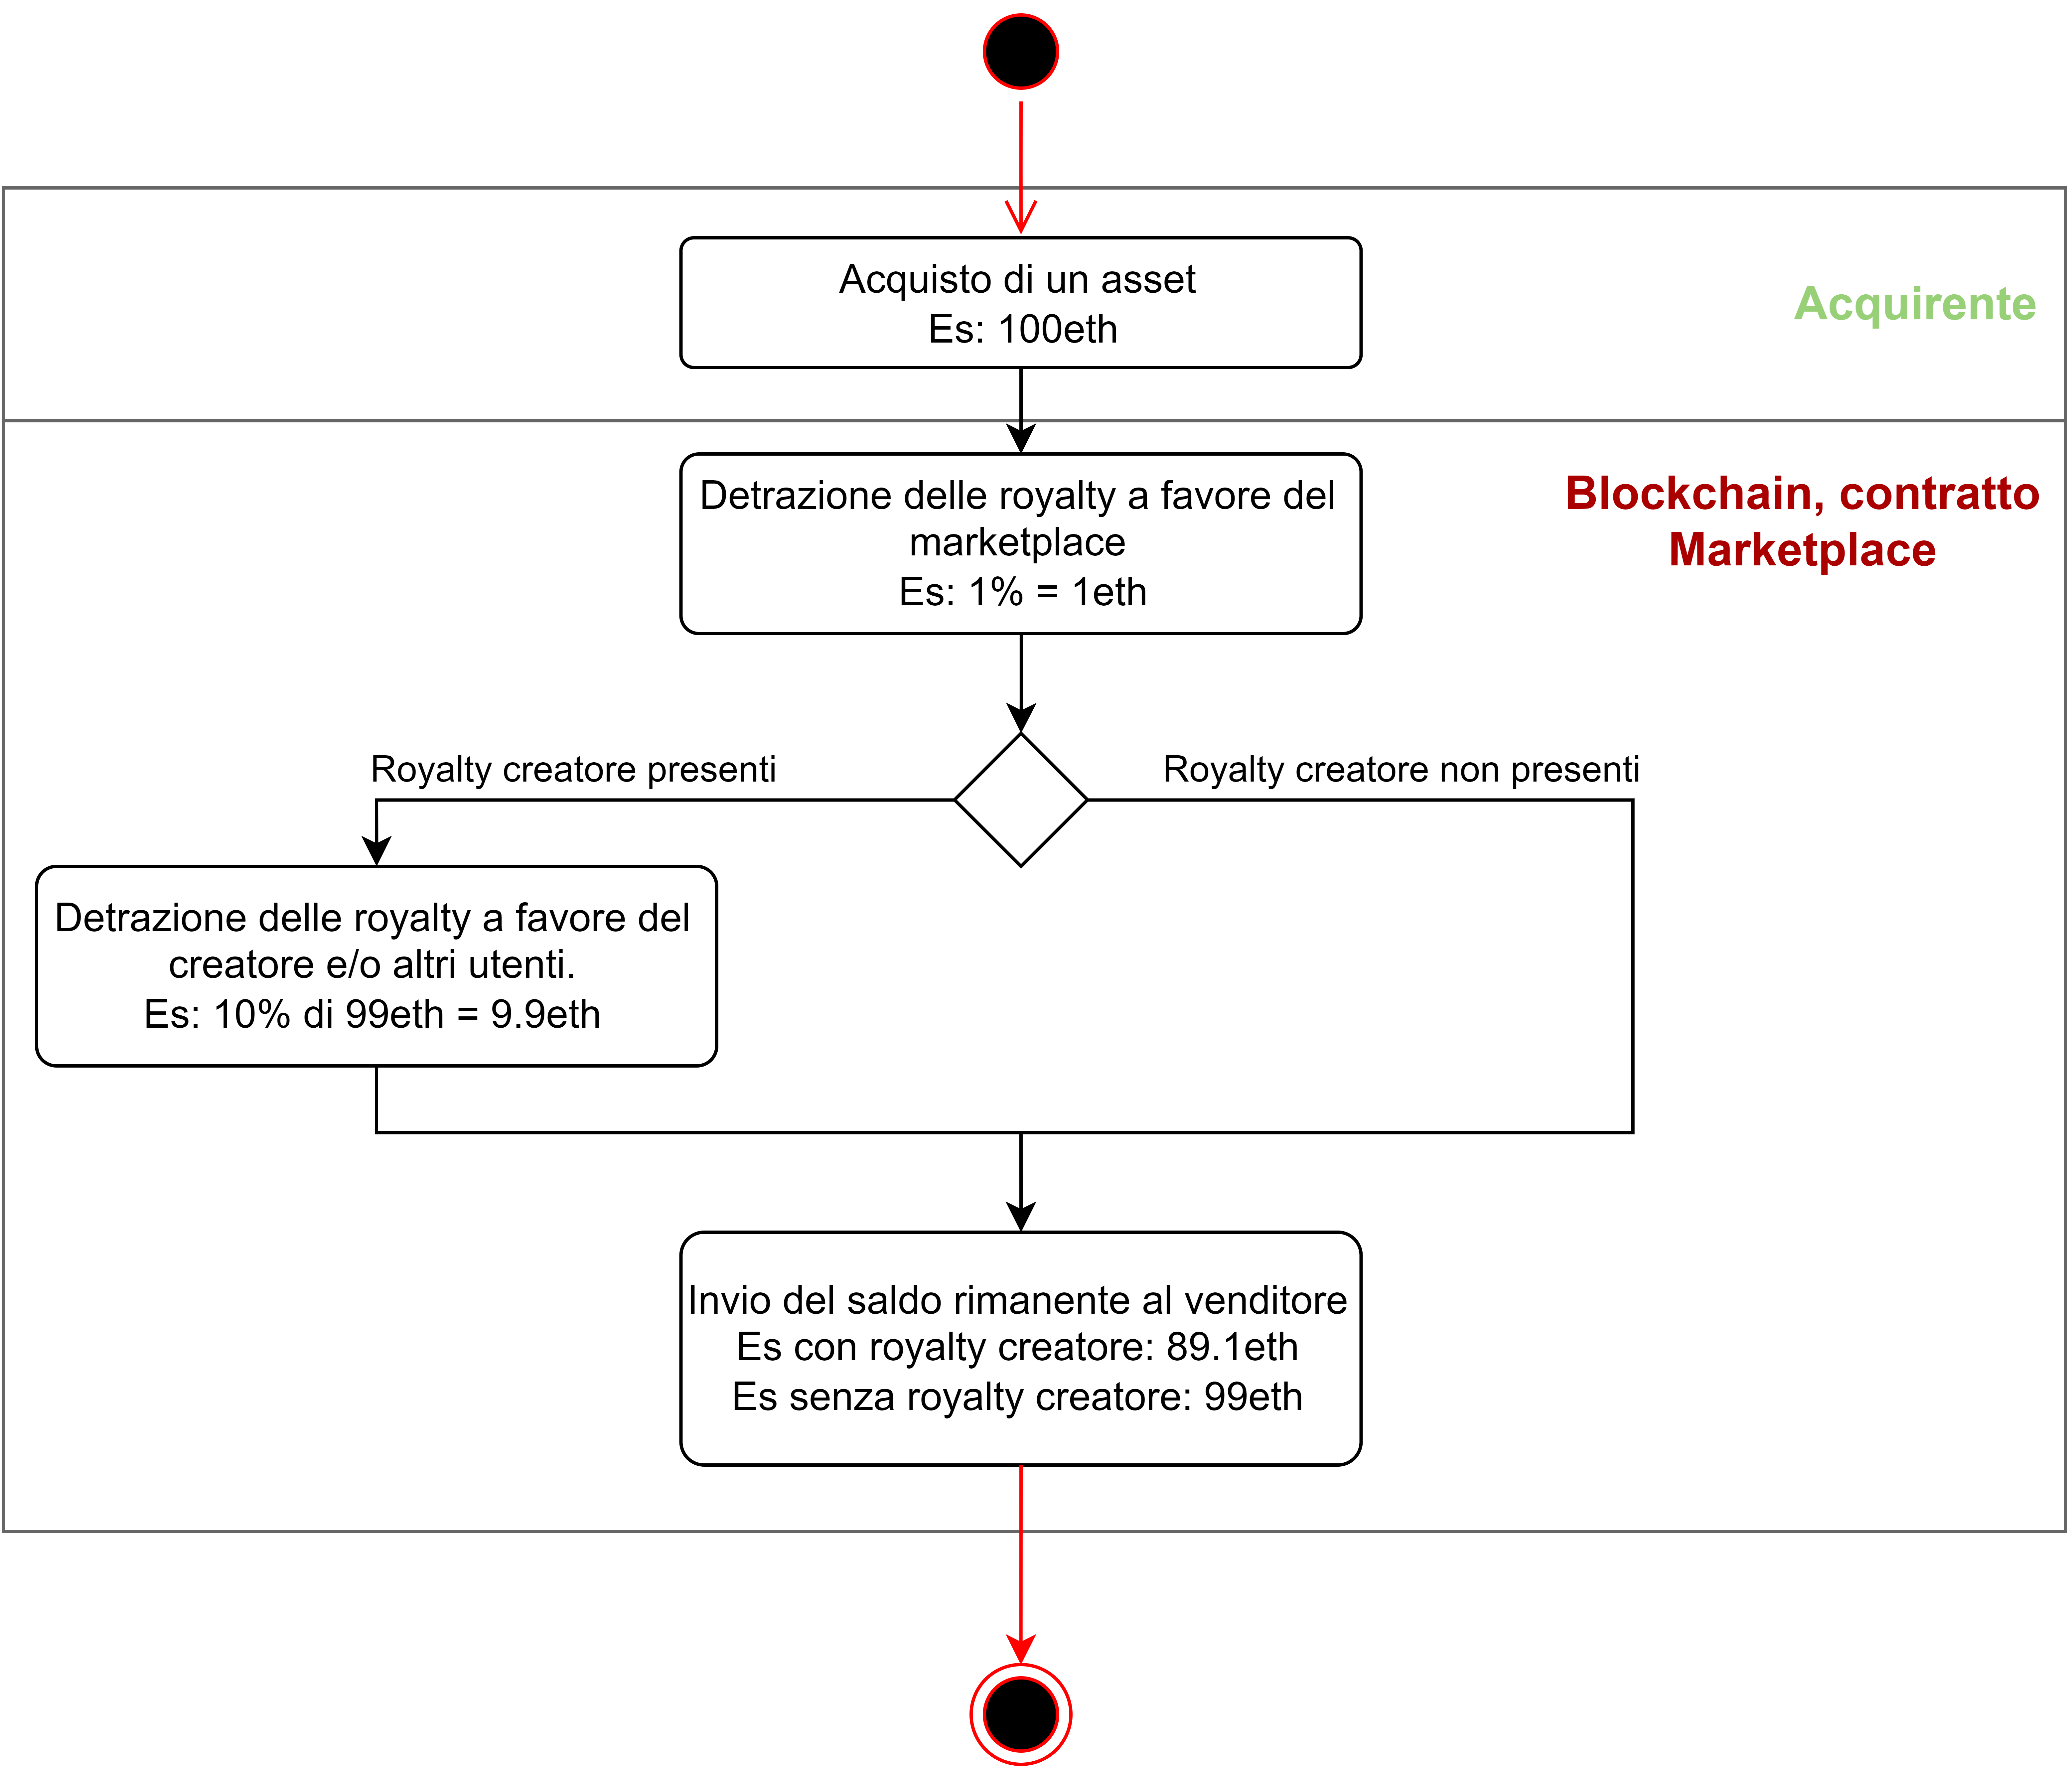
\includegraphics[width=0.8\textwidth]{images/SuddivisioneRoyalty.png}
    \caption{Suddivisione del revenue share}
    \label{fig:distribuzione-royalty}
\end{figure}



\subsection{Marketplace revenue share}
Come sarà approfondito nel capitolo \hyperref[sec:smart-contract-shopychange]{\textit{Blockchain - Smart contracts}}, il contratto principale del marketplace è composto da più moduli che si occupano di gestire le varie funzionalità di esso.

In particolare, il modulo \textit{MarketplaceEarnable} si occupa di gestire il \textit{revenue share} del marketplace, le sue funzionalità sono:

\begin{itemize}
    \item Salvare la percentuale di \textit{revenue share} a favore del marketplace.
    \item Fornire metodi di lettura e scrittura della percentuale di \textit{revenue share}, nonchè del calcolo del \textit{revenue share} in base al prezzo di vendita di un asset.
    \item Fornire metodi di ritiro dell'ammontare ottenuto dalle varie vendite.
\end{itemize}

Tramite queste funzionalità l'utente amministratore ha la possibilità di modificare e ritirare il \textit{revenue share} in qualsiasi momento. Per semplicità, è stata sviluppata un'interfaccia grafica che permette l'interazione con lo \textit{smart contract}, analizzata più in dettaglio nel capitolo \hyperref[sec:admin-dashboard]{\textit{Admin Dashboard}}.

\subsection{Creator / Users revenue share}
La ripartizione del \textit{revenue share} a favore del creatore risulta più complessa, essendo un tema attualmente in fase di sviluppo con diverse soluzioni proposte.

Il problema nasce dal fatto che non esiste uno standard ad oggi largamente utilizzato, il che ha portato i marketplace a sviluppare soluzioni proprietarie e non interoperabili tra loro. 

La causa principale di questa mancanza è a livello implementativo, non è possibile sapere se l'asset è stato acquistato tramite un marketplace o se il possessore abbia deciso di cederlo, dove in quest'ultimo caso il \textit{revenue share} non dovrebbe essere applicato.
Più in dettaglio, nel momento in cui avviene la chiamata ai diversi metodi di \textit{transfer}, definiti negli standard \textit{ERC721} e \textit{ERC1155}, il valore inviato con la transazione (ovvero il prezzo di vendita) non è accessibile, in quanto i metodi di \textit{transfer} sono di tipo \textit{non payable}, ovvero non permettono di inviare ETH. 

Perciò, per risolvere questo problema sono state analizzate le soluzioni implementate da due dei marketplace più famosi e utilizzati, cioè \textit{OpenSea}\footnote{https://opensea.io/} e \textit{Rarible}\footnote{https://rarible.com/}.

\begin{itemize}
    \item \textit{OpenSea} \cite{operator-filter-registry}: la soluzione da loro adottata si basa su smart contracts.
    In particolare, su un registro distribuito chiamato \textit{Operator Filter Registry} che permette di definire una lista di indirizzi abilitati alla gestione degli \textit{assets}. 

    Il creatore di una collezione dovrà modificare il proprio contratto  \textit{ERC721} o \textit{ERC1155} per risultare compatibile. Tramite questa modifica il nuovo contratto delegherà il controllo degli operatori approvati all'\textit{Operator Filter Registry}.

    L'\textit{enforcement}, ovvero il controllo che le \textit{revenue share} siano ripartite nel modo definito, avviene semplicemente con il fatto che, i marketplace riconosciuti per \textbf{non} applicare il \textit{revenue share} vengono inseriti in una \textit{blacklist} e quindi non possono gestire gli \textit{assets}.

    Il registro distribuito, inizialmente gestito e popolato da OpenSea, è ora gestito dal gruppo \textit{Creator Ownership Research Institute} (CORI).

    In aggiunta, i marketplace che sono riconosciuti per applicare il \textit{revenue share} hanno la possibilità di implementare il sistema di \textit{revenue share} a loro piacimento.
    \item \textit{Rarible} \cite{rarible-community-marketplaces}: la soluzione implementata da Rarible consiste anch'essa in un registro distribuito tra una lista di marketplace creati con l'aiuto di Rarible stesso, questo gruppo è chiamato \textit{Community Marketplaces}.
\end{itemize}

Le soluzioni implementate da OpenSea e Rarible sono molto simili, tuttavia presentano problemi di interoperabilità. Nel momento in cui un creatore decidesse di utilizzare uno dei due marketplace, dovrebbe ripetere la stessa configurazione nell'altro mercato digitale. Inoltre, potrebbe essere necessario modificare anche lo \textit{smart contract} così da risultare compatibile, il che potrebbe essere un problema per i creatori meno esperti. Purtroppo però, anche con gli accorgimenti sopra descritti, non è possibile garantire che il \textit{revenue share} venga applicato correttamente in altri marketplace.

Riassumendo, la gestione di \textit{revenue share} presenta due principali problematiche:
\begin{enumerate}
    \item \textit{Interoperabilità}: Non esiste uno standard largamente utilizzato e quindi non è possibile garantire l'interoperabilità tra i diversi marketplace
    \item \textit{Enforcement}: Non è possibile essere sicuri che il \textit{revenue share} venga applicato correttamente, essendo un'azione che deve essere effettuata in modo volontario dal marketplace 
\end{enumerate}

I due problemi sopra descritti hanno soluzioni non compatibili tra loro. Analizzando più in dettaglio le soluzioni proposte da OpenSea e Rarible, è possibile notare che entrambe presentano un registro distribuito che permette di definire una lista di marketplace abilitati alla gestione degli \textit{assets}, tuttavia risulta essere un gruppo chiuso, non rispecchiando l'ideologia di decentralizzazione. D'altronde, in caso di gruppo aperto ed essendo il pagamento di \textit{revenue share} un'azione volontaria, non è possibile garantire che il \textit{revenue share} venga applicato correttamente.

Nei prossimi capitoli verranno analizzate in maniera più approfondita le soluzioni proposte.

\subsubsection{Utilizzo di ERC2981 e PaymentSplitter}
\label{sec:utilizzo-erc2981-payment-splitter}

La prima soluzione implementata nel marketplace \textit{Shopychange}, include l'utilizzo di una variante dello standard ERC2981. Come descritto nel capitolo \hyperref[sec:erc2981]{\textit{ERC2981}}, questo standard permette di aggiungere le informazioni relative al \textit{revenue share} all'interno del contratto \textit{ERC721} o \textit{ERC1155}. Tuttavia, presenta un importante limitazione, è il marketplace stesso che deve recuperare le informazioni relative al \textit{revenue share} e applicarlo.

In aggiunta, è possibile definire un solo destinatario di \textit{revenue share}, il che potrebbe essere un problema nel caso in cui il creatore volesse distribuire il guadagno tra più utenti. 

Per risolvere questo problema, lo studente ha proposto un nuovo standard definito con il nome \textit{ERC2981MultiReceiver}, il quale permette di definire più destinatari. A livello implementativo è stato utilizzato il contratto \textit{PaymentSplitter}, il quale consente di definire più destinatari e di ripartire il guadagno in base alla percentuale scelta per ogni partecipante. Maggiori informazioni saranno fornite nel capitolo \hyperref[sec:erc2981-multi-receiver]{\textit{ERC2981MultiReceiver}}.

La soluzione proposta risolve il problema di interoperabilità tra i diversi marketplace utilizzando lo standard emergente \textit{ERC2981} e permette di definire più destinatari. Ciononstante, non risolve il problema di \textit{enforcement} del \textit{revenue share}.
Attraverso la figura \ref{fig:creazioneVenditaNFTRoyaltyERC2981MultiReceiver} è possibile osservare il processo di creazione di un NFT (o collezione) con la rispettiva vendita con \textit{revenue share}.

\begin{figure}[H]
    \centering
    \includegraphics[width=0.9\textwidth]{images/creazioneVenditaNFTRoyaltyERC2981MultiReceiver.png}
    \caption{processo di creazione e vendita di un NFT con ERC2981MultiReceiver}
    \label{fig:creazioneVenditaNFTRoyaltyERC2981MultiReceiver}
\end{figure}


\subsubsection{Override del metodo transfer}

La seconda soluzione analizzata, consiste nell'override del metodo \textit{transfer} definito negli standard \textit{ERC721} e \textit{ERC1155}. In maniera più approfondita, è stato creato un ulteriore modulo definito come \textit{ERC721EnforceRoyalty}, il quale permette di definire le informazioni di \textit{revenue share}, ovvero il destinatario con la relativa percentuale e il prezzo dell'asset. Le operazioni necessarie per effettuare un \textit{transfer} sono le seguenti:

\begin{enumerate}
    \item Il creatore della collezione deve definire il destinatario e la percentuale di \textit{revenue share} per ogni asset (o per la collezione)
    \item Il possessore dell'asset imposta un prezzo di vendita
    \item L'acquirente deve inviare l'ammontare relativo al \textit{revenue share} al contratto, il quale si occuperà di salvare il valore e sbloccare il \textit{transfer}
    \item L'acquirente o il marketplace approvato effettua il \textit{transfer} dell'asset
    \item Automaticamente l'ammontare del \textit{revenue share} viene inviato al destinatario
\end{enumerate}

La soluzione analizzata risolve il problema di \textit{enforcement}, in quanto il metodo \textit{transfer} viene bloccato finchè non viene inviato l'ammontare del \textit{revenue share}. Essendo che l'interoperabilità non è garantita, la soluzione potrebbe essere adatta a marketplace che non hanno o non vogliono offrire la possibilità di acquistare asset tramite altri marketplace. Un esempio di questo tipo, potrebbe essere un mercato digitale specializzato nella vendita di asset relativi a biglietti di ingresso ad eventi. Nei quali si vuole garantire che il biglietto non venga rivenduto ad un prezzo superiore a quello originale.

Attraverso la figura \ref{fig:creazioneVenditaNFTOverride} è possibile osservare il processo di creazione di un NFT (o collezione) con la rispettiva vendita con \textit{revenue share} tramite override del metodo \textit{transfer}.

\begin{figure}[H]
    \centering
    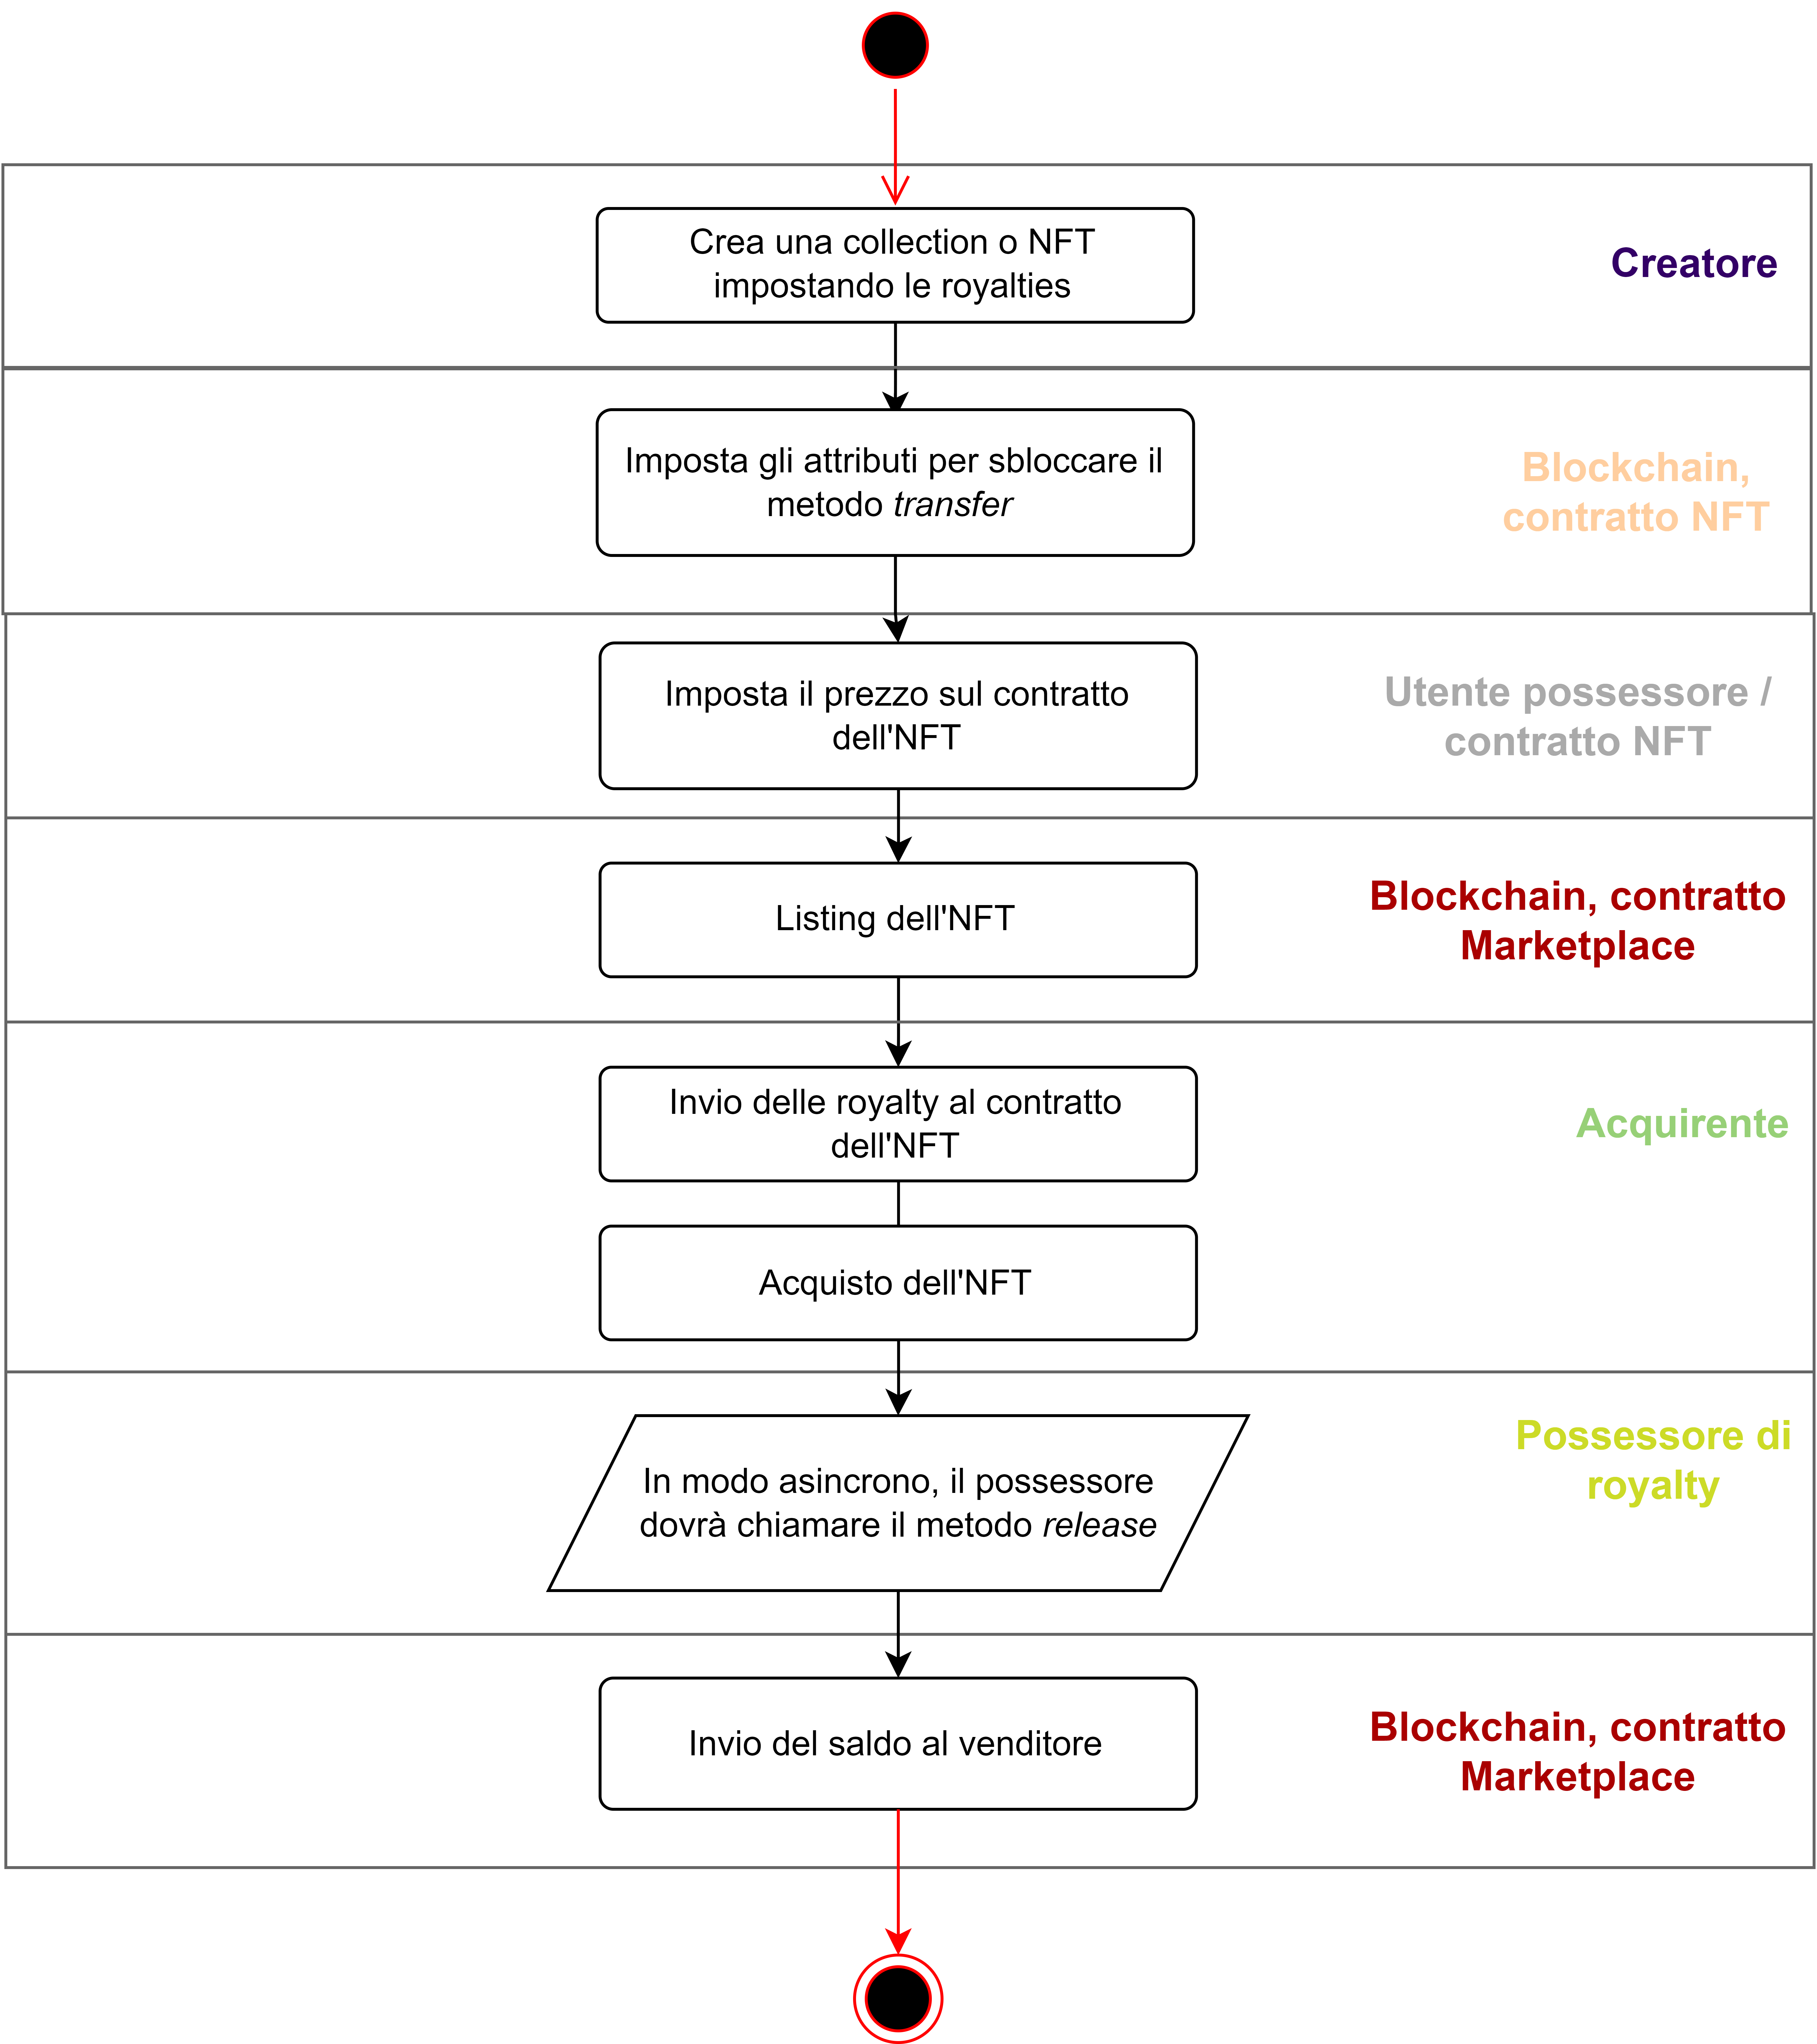
\includegraphics[width=1\textwidth]{images/creazioneVenditaNFTOverride.png}
    \caption{processo di creazione e vendita di un NFT con override del metodo transfer}
    \label{fig:creazioneVenditaNFTOverride}
\end{figure}

\newpage